\documentclass{article}

% if you need to pass options to natbib, use, e.g.:
% \PassOptionsToPackage{numbers, compress}{natbib}
% before loading nips

% ready for submission
%\usepackage{sty_bst/nips}

% to compile a preprint version, e.g., for submission to arXiv, add
% add the [preprint] option:
%\usepackage[preprint]{sty_bst/nips}

% to compile a camera-ready version, add the [final] option, e.g.:
\usepackage[final]{sty_bst/neurips_2018}

% to avoid loading the natbib package, add option nonatbib:
% \usepackage[nonatbib]{sty_bst/nips}

\usepackage[utf8]{inputenc} % allow utf-8 input
\usepackage[T1]{fontenc}    % use 8-bit T1 fonts
\usepackage{hyperref}       % hyperlinks
\usepackage{url}            % simple URL typesetting
\usepackage{booktabs}       % professional-quality tables
\usepackage{amsfonts}       % blackboard math symbols
\usepackage{nicefrac}       % compact symbols for 1/2, etc.
\usepackage{microtype}      % microtypography
\usepackage{booktabs} % for professional tables
\usepackage{amsmath}
\usepackage{amssymb}
\usepackage{color}
\usepackage{verbatim}
\usepackage{graphicx}
\usepackage{wrapfig}
\usepackage{subfig}
\usepackage{multirow}
\newcommand{\todo}[1]{\textcolor{red}{#1}}
\usepackage{xspace}
\newcommand{\Petridish}{Petridish\xspace}

\title{Macro Neural Architecture Search Revisited}

% The \author macro works with any number of authors. There are two
% commands used to separate the names and addresses of multiple
% authors: \And and \AND.
%
% Using \And between authors leaves it to LaTeX to determine where to
% break the lines. Using \AND forces a line break at that point. So,
% if LaTeX puts 3 of 4 authors names on the first line, and the last
% on the second line, try using \AND instead of \And before the third
% author name.

%\author{
%Hanzhang Hu\thanks{This work was part of an internship at Microsoft Research by Hanzhang Hu.},  
%Martial Hebert, 
%J. Andrew Bagnell \\
%Carnegie Mellon University, 
%Pittsburgh, PA \\
%\texttt{\{hanzhang,hebert,dbagnell\}@cs.cmu.edu} 
%\And
%John Langford,
%Rich Caruana,
%Eric Horvitz,
%Debadeepta Dey \\
%Microsoft Research \\
%\texttt{\{jcl,rcaruana,horvitz,dedey\}@microsoft.com} \\
%}

\author{
Hanzhang Hu$^{1}$\thanks{This work was part of an internship at Microsoft Research by Hanzhang Hu.}, John Langford$^{2}$, Rich Caruana$^{2}$, Eric Horvitz$^{2}$, Debadeepta Dey$^{2}$  \\
$^{1}$Carnegie Mellon University; $^2$Microsoft Research \\
\texttt{hanzhang@cs.cmu.edu},  \texttt{\{jcl,rcaruana,horvitz,dedey\}@microsoft.com} 
}

\begin{document}
% \nipsfinalcopy is no longer used

\maketitle

\begin{abstract}
Neural architecture search (NAS) has recently shown promising results for automatically finding cost-efficient and accurate predictors. However, most recent work exclusively study the small search space of repeatable network modules (cells), instead of the more general overall network (macro), partially because the models found by macro-search typically require an order of magnitude more parameters compared to cell-search to have the same accuracy. In this work, we show through ablation study that this gap mainly exists due to the difference in initial models. In fact, by starting with the same condition as cell-search, the proposed macro-search can find a CIFAR-10 model that has 2.93\% test error rate and uses 3.1 million parameters. Our macro-search algorithm has the advantage of being simple and fast. The search procedure randomly and incrementally grows the most cost-efficient models on the Pareto frontier. The proposed search takes only 6 GPU-days, which is much smaller than those of many existing methods, while achieving comparable or better results. 
\end{abstract}

\section{Introduction and Background}
\label{sec:introduction}
There has been keen interest in automated neural architecture search (NAS), ever since \citet{NAS} showed that it is possible to find models that are more accurate and less computationally expensive than the best human designed models. While early NAS work~\citep{NAS,Real2017EvoNet} consider \textbf{macro-search}, where each layer in the network can take inputs from any previous layer independent of how other layers choose their inputs, the most recent work~\citep{Liu2018DARTSDA,NAONet,CaiPathLevel} only consider \textbf{cell-search}, where the algorithm only searches over how a few layers (typically $5\sim8$) are connected to each other, and use the found connection pattern, called a cell, as a repeatable module in a human designed skeleton network that consists of a sequence of cells. Macro-search and cell-search are compared in~\citep{NASCell,Liu2017ProgressiveNA,Pham2018EfficientNA,Elsken2018EfficientMN}, which find that in comparison to macro-search, cell-search can find models that are more accurate with an order of magnitude fewer parameters. ~\citet{NASCell} also demonstrate that cells found on CIFAR-10 can be composed with larger skeleton outer networks to become state-of-the-art models on ImageNet~\citep{ILSVRC15}.
Thereafter, no attempts have been made to reconcile the gap between macro and cell-search in terms of the performance of the found models, despite the fact that macro-search is more general and may be the only option on novel tasks and data-sets where expert knowledge about the outer skeleton does not exist. 

In this work, we investigate why macro-search has been outperformed by cell-search, and find that the discrepancy in the initial model to be a dominating factor. In particular, when we start macro-search with the outer skeleton of~\citet{NASCell} composed with one of the simplest cells in their search space, our macro-search found models for CIFAR-10 that takes 3.1 million parameters to reach 2.93\% test error (averaged over 5 trials). This is close to the state-of-the-art, which is previously only achievable by cell-search, and to the best of our knowledge, it is the best macro-search result at the time of writing. The search is also much faster than many existing methods, taking only 6 GPU-days. 
Our ablation study then shows that macro-search actually finds slightly better models than cell-search if they start with the same model. Furthermore, if we reduce the starting model complexity by half, then our macro-search result is degraded to 3.44\% even when we triple the search resource. This sheds light on the current macro-cell gap: though macro-search can potentially utilize the extra freedom to find better models than cell-search, the benefits are overshadowed currently, because cell-search methods uses better initial models. 

\section{Search via Random Growth from Promising Models}
\label{sec:search_algorithm}

We propose a simple algorithm, \textbf{\Petridish}, to grow networks in search of cost-efficient models. The search is defined by five components: the choice of parent models, the incremental model changes, the training procedure during search, the initial model, and the procedure for training the final model. The first three components are repeatedly looped over by parallel workers. The best model in validation goes through the final training procedure to report test error. We give a brief overview below:

\begin{wrapfigure}{R}{0.32\textwidth}
\centering
    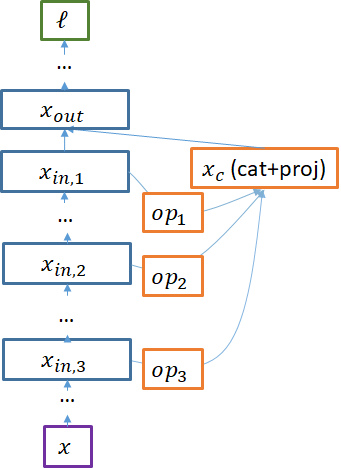
\includegraphics[width=0.3\textwidth, keepaspectratio]{img/hallu_soft.png}
    \caption{Incremental model change. Blue indicates existing layers, orange indicates increments. $op_i$ are considered part of $x_c$.}
    \label{fig:hallu_soft}
\end{wrapfigure}

\textbf{Choice of Parent models.}
\label{sec:choose_parent}
The goal of our algorithm is to find \emph{cost-efficient} predictors. For simplicity, we take a greedy approach. Whenever we need to choose a parent model, we first plot the computational cost versus validation error of existing models, and then compute the lower convex hull of this curve. We stop the hull when it starts increasing. We then choose a model on the hull as the parent with probability defined as the following.
If $m_1$ and $m_2$ are two adjacent models on the hull, with computational costs $c_1$ and $c_2$ ($c_1 < c_2$), then we set the probability weight of $m_1$ to be proportional to $c_2 - c_1$. The most accurate model (which has no following model on the curve) is always chosen with probability 0.5. This greedy approach is most similar to multi-objective architecture search~\citep{Elsken2018EfficientMN, Hsu2018MONASMN} that focuses on models on the pareto-frontier of the performance scatter plot. Both methods modify the most cost-efficient models and convex hull is a subset of the pareto-frontier.

\textbf{Incremental Model Change.}
\label{sec:candidate_layers}
Fig.~\ref{fig:hallu_soft} illustrates a single incremental model change, $x_c$. Every iteration we randomly generate many of them. The number of changes at each iteration depends on the initial network, and we detail the relation later. To form $x_c$, we first randomly sample the target layer $x_{out}$ from layers that were in the initial network. Then three input layers $x_{in,i}$ for $i=1,2,3$ are chosen. To ensure that $x_c$ has access to local layers, $x_{in,1}$ always chooses the deepest input of $x_{out}$ that was in the initial network. $x_{in,2}$ and $x_{in,3}$ are sampled with replacement uniformly at random from all layers that are topologically earlier than $x_{out}$.
Each input layer then uniformly randomly choose one of the five operations: 3x3 and 5x5 separable convolution, 3x3 max and average pooling, and identity. Following~\citep{NASCell,Real2018RegularizedEF,Pham2018EfficientNA}, separable convolutions are applied twice. 
The processed inputs are concatenated together and then projected to the same shape as the target layer $x_{out}$ using a 1x1 convolution. The result is the incremental change $x_c$, which is added to $x_{out}$. 

In our cell-search, our baseline, we use the same sampling procedure to form the incremental changes, except that we follow~\citep{NASCell} and choose inputs within the same cell or from the outputs of the previous two cells in cell-search.

\textbf{Training During Search on CIFAR-10.}
\label{sec:search_training}
The incremental changes have randomly initialized parameters while the parameters of the parent model are reused. We train the new network (parent network + incremental changes) with a batch size of 32 using SGDR~\citep{cosine_lr} that starts at 0.025 and ends at 0 in 80 epochs for two cycles (160 epochs). Following~\citep{Elsken2018EfficientMN}, we apply standard data augmentations of cropping-after-padding, left-right flipping, and pixel-wise normalization, along with cutout~\citep{cutout}.

\textbf{Initial Network.} 
\label{sec:init_network}
Since we aim to compare cell and macro-search, we start with a network that is compatible with both. Following common baselines~\citep{NASCell}, we start on a network that has 3 blocks. Each block has $N=6$ regular cells and there is a reduction cell in between blocks.
The initial channel size is $F=32$. Our initial cell is inspired by ResNet's~\citep{resnet} residual unit: given an input $x$, it produces $h(x) + x$, where $h$ is the 3x3 separable convolution operation in our search space. This cell is also the smallest non-trivial cell in the search space of~\citep{NASCell}. 
At the start of each search, the initial model is trained from scratch as if it is a final model (more details below). The initial model has around 4.6\% error rate on CIFAR-10. 
We recognize that this initial model for macro-search is more complex than early pioneering work~\citep{NAS,Real2017EvoNet}. Hence, we also conduct an ablation study using $N=3$ for macro-search, and we find that this discrepancy in initial models is a crucial reason for macro-search to be outperformed by cell-search in current literature. 

We choose one increment for each of normal and reduction cells in cell-search. Since there are $(N\times 3 + 2=)20$ cells, we choose 20 increments for macro-search, so that the overall number of structural increments is kept the same at each iteration for comparing macro and cell-search fairly.



\vspace{-3pt}
\section{Experiments}
\label{sec:experiment}
\vspace{-3pt}
\begin{table}[t]
    \centering
    \caption{Comparison against state-of-the-art recognition results on CIFAR-10. Results marked with $\dagger$ are not trained with cutout. The first block represents approaches for macro-search. The second block represents approaches for cell-search. 
    }
    \begin{tabular}{l|cccc}
    \hline
\multirow{ 2}{*}{\textbf{Method} }
        &  \textbf{\# params} 
        &  \textbf{Search } 
        &  \textbf{Test Error } \\
        &  (mil.)
        &  (GPU-Days)
        &  (\%)\\
\hline
\citet{NAS}$^{\dagger}$
    &  7.1 &  1680+ &  4.47  \\
\citet{NAS} + more filters$^{\dagger}$
    &  37.4 &   1680+ &  3.65   \\
\citet{Real2017EvoNet}$^{\dagger}$
    &  5.4 &   2500 &  5.4  \\
ENAS macro~\citep{Pham2018EfficientNA}$^{\dagger}$
    &  21.3 &  0.32 &  4.23 \\
ENAS macro + more filters$^{\dagger}$
    &  38 &   0.32 &  3.87 \\
Lemonade I~\citep{Elsken2018EfficientMN}
    &  8.9 &    56 &  3.37 \\
\hline
\Petridish initial model ($N=6$, $F=32$)
    & 0.4 &  -- & 4.6 \\
%\Petridish macro without DropPath
%    & 3.1 & 6 & 3.38 \\
\textbf{\Petridish macro} 
    & \textbf{4.8} & \textbf{27.2} & \textbf{2.86} \\
%\Petridish macro (start at $N$=3, $F$=32)
%    & 2.7 & 18 & 3.44 \\
\hline \hline
NasNet-A~\citep{NASCell}
    &  3.3 &    1800 &  2.65   \\
AmoebaNet-A~\citep{Real2018RegularizedEF}
    &  3.2 &  3150 &  3.3  \\
AmoebaNet-B~\citep{Real2018RegularizedEF} 
    &  2.8 &   3150 &  2.55 \\ 
PNAS~\citep{Liu2017ProgressiveNA}$^{\dagger}$
    &  3.2 &  225 &  3.41 \\
Heirarchical NAS~\citep{Liu2018HierNA}$^{\dagger}$
    &  15.7 &    300 &  3.75 \\ 
ENAS cell~\citep{Pham2018EfficientNA}
    &  4.6 &  0.45 &  2.89 \\ 
ENAS cell~\citep{Pham2018EfficientNA}$^{\dagger}$
    &  4.6 &  0.45 &  3.54 \\ 
Lemonade II~\citep{Elsken2018EfficientMN}
    &  3.98 &  56 &  3.50 \\
Darts~\citep{Liu2018DARTSDA}
    &  3.4 &   4 &  2.83 \\ 
Darts random~\citep{Liu2018DARTSDA}
    & 3.1 & -- & 3.49 \\
\citet{CaiPathLevel} 
    & 5.7 &  8  & 2.49 \\
\citet{NAONet}$^{\dagger}$
    & 3.3 & 0.4 & 3.53 \\
\hline
\textbf{\Petridish cell}
    & \textbf{2.8} & \textbf{15.3} & \textbf{2.79} \\
%\Petridish cell + more filters
%    & 3.5 & 6 & 3.05 \\
\hline
    \end{tabular}
    \label{tab:cifar10_search}
\end{table}



\begin{table}[t]
    \centering
    \caption{Comparison against recognition results on CIFAR-100. \Petridish models are the ones found in CIFAR-10 search. The first block represents the best human designed models. The second represents models found through automated macro-search on CIFAR100. 
    }
    \begin{tabular}{l|ccc}
    \hline
\multirow{ 2}{*}{\textbf{Method} }
        &  \textbf{\# params} 
        &  \textbf{Test Error } \\
        &  (mil.)
        &  (\%)\\
\hline
DenseNet-BC (k=40)~\citep{densenet}
    & 25.6 & 17.18 \\
Shake-Shake~\citep{shakeshake}
    & 26.2 & 15.85 \\
\hline
SMASHv2~\citep{SMASH}
    & 16 & 20.6 \\
\citet{Real2017EvoNet}
    & 40.4 & 23.7 \\
\citet{elskenSimpleNAS}
    & 22.3 & 23.4 \\
Block-QNN-S~\citep{blockqnn}
    & 6.1 & 20.65 \\
\hline
\textbf{\Petridish macro}
    & \textbf{4.8} & \textbf{18.50} \\
\hline
\textbf{\Petridish cell}
    & \textbf{2.8} & \textbf{19.08} \\
\hline
    \end{tabular}
    \label{tab:cifar100_search}
\end{table}

Our experiments first showcase that macro-search can indeed find state-of-the-art models on CIFAR-10 that are currently only obtained via cell-search. Then we show that \Petridish macro-search can outperform \Petridish cell-search if they start from the same model. Finally, we use ablation study on the initial model to show how dominating initial model effects are on the search results.  

\textbf{Final training of the best models obtained.} 
Following~\citep{NAS,NASCell,Real2018RegularizedEF}, we train from scratch the best models obtained via the search procedure (in terms of validation error), with batch size 32 using cosine learning rate that shrinks from 0.025 to 0 in 600 epochs. We apply path drop-out~\citep{larsson2016fractalnet} for the final training. Both training and validation data are used. We report the average test error of five independent training runs.

\textbf{CIFAR-10 macro-search.}
\Petridish macro-search is run on 4 GPUs for 1.5 days for a total of 6 GPU-days.
%We have three independent runs of \Petridish macro-search, each having 4 GPUs for 1.5 days, so a total of 18 GPU days. 
Table~\ref{tab:cifar10_search} displays for each automated search method the number of parameters in the final obtained model, search cost in GPU-days, and the test error on CIFAR-10. \Petridish macro-search achieves much lower error rate (2.93\%) than \emph{all  previous macro-search based methods} (first block of Table~\ref{tab:cifar10_search}), and only requires a fraction of parameters. In fact, the final obtained model is close to the state-of-the-art that is currently only achieved by cell-search based methods, which are listed in the second block of Table~\ref{tab:cifar10_search}.

\textbf{Comparison to cell-search.}
\Petridish macro and cell-searches start with the same model and are constrained to make the same amount of change to the overall model at each step. In Table~\ref{tab:cifar10_search}, our macro-search outperforms cell-search by finding a more accurate and less expensive model (2.93\% vs. 3.05\%), indicating that the extra freedom of macro-search can indeed help find better models.


%The comparison to state-of-the-art models is more nuanced. 
%We use the same skeleton as~\citep{NASCell,Real2018RegularizedEF}, but they have 100x search time. 
%~\citep{Pham2018EfficientNA, Liu2018DARTSDA} also use the same skeleton, and have similar final performance. However, as their final model is a sub-graph of their initial super-graph, their initial performance should be from random sub-graphs. 


\textbf{The importance of initial model.}
\Petridish is the closest to~\citep{Elsken2018EfficientMN}, since both work warm start from existing models that are the most cost-efficient, and incrementally modify the networks at random. One major difference is the starting model. \citet{Elsken2018EfficientMN} starts at shallow models with three conv layers. \Petridish starts at one of the simplest model that the cell-search can start with, but it is still vastly more complex than the starting models of previous macro-search. 
In fact, when we set $N=3$ instead of $N=6$ in the initial model, we observe in Table~\ref{tab:cifar10_search} that the found model only achieves 3.44\% error rate, even if we increase the search resource to 18 GPU-days. This suggests that the effect of initial model far outweighs the difference between macro and cell-searches, which only causes a change of 0.1\% in error rates. 
We can further infer the impact of initial models from other existing works. For instance,~\citep{NASCell,Real2018RegularizedEF,Pham2018EfficientNA,Liu2018DARTSDA,NAONet} all use the same or similar skeletons, and their results are similar.
\footnote{~\citep{NASCell,Real2018RegularizedEF} have similar performance, but are better than the others partially due to the thousands of GPU-days spent. ~\citep{Pham2018EfficientNA,Liu2018DARTSDA,NAONet} have fast search, because of parameter sharing during search, a topic outside the scope of this work.}
By starting from a more complex skeleton and a more complex starting cell\footnote{\citep{CaiPathLevel} sets $N=8$, and the starting cell is PyramidNet~\citep{pyramidnet}}, \citep{CaiPathLevel} finds a more accurate model using only 8 GPU-days. 


\textbf{Transfer to other data-sets.}
We also display in Table~\ref{tab:cifar100_search} the performance of human designed and macro-search models on CIFAR-100. Our model found in macro-search on CIFAR-10 achieves better accuracy than published macro-search results on CIFAR-100. We also transfer the macro-search model to ILSVRC2012~\citep{ILSVRC15} (more detail in appendix), and achieves 27.2\% top-1 error rate using 6.88 million parameters and 830 million multi-add operations.

\vspace{-3pt}
\section{Discussion and Ongoing Work}
\label{sec:conclusion}
\vspace{-3pt}
The ablation study on initial models shows that they are extremely impactful to search speed and final model accuracy, we encourage future work to report initial model performances for fair evaluation of search algorithms. 
The successful macro-search on CIFAR-10 through \Petridish and ablation study on macro and cell-search together point future work to reconsider macro-search, because it is more general, and it may be the only viable option on novel data-sets and tasks where a reasonable outer skeleton architecture may not be available.



\bibliographystyle{sty_bst/icml.bst}
\bibliography{network_search}

\newpage
\appendix

\section{Transfer of Macro-search Model to ILSVRC2012}


\begin{table}[t]
    \centering
    \caption{ILSVRC2012 transfer results. 
    }
    \begin{tabular}{l|cccc}
    \hline
\multirow{ 2}{*}{\textbf{Method} }
        &  \textbf{\# params} 
        &  \textbf{\# multi-add}
        &  \textbf{top-1 Test Error } \\
        &  (mil.)
        &  (mil.)
        &  (\%)\\
\hline
Inception-v1 (Szegedy et al., 2015)
    & 6.6 & 1448 & 30.2 \\
MobileNetV2 (Sandler et al., 2018)
    & 6.9 & 585 & 28.0 \\
\hline
NASNet-A (Zoph et al., 2017) 
    & 5.3 & 564 & 26.0 \\
NASNet-B (Zoph et al., 2017) 
    & 5.3 & 488 & 27.2 \\
AmoebaNet-A (Real et al., 2018)
    & 5.1 & 555 & 25.5 \\
PNAS (Liu et al., 2017a)
    & 5.1 & 588 & 25.8 \\
DARTS (Liu et al., 2018)
    & 4.9 & 595 & 26.9 \\
\hline
\textbf{\Petridish macro} 
    & \textbf{10.4} & \textbf{1247} & \textbf{25.2} \\
\hline
\textbf{\Petridish cell}
    & \textbf{6.2} & \textbf{813} & \textbf{25.4} \\
\hline
    \end{tabular}
    \label{tab:imagenet_compare}
\end{table}

For ILSVRC2012~\citep{ILSVRC15}, we take the standard data augmentation approach of~\citep{resnet}, and use 224x224 input images. Since our macro-search is performed on CIFAR10, which consists of 32x32 images, the found models are not directly applicable to ILSVRC2012. Instead we add three reductions at the start of the model so the 224x224 images of ILSVRC2012 are reduced to 28x28. First, a 3x3 conv with stride of two projects the RGB-color feature into 12 channels. Then we apply two simple reduction cells, each of which is the same as the reduction cells in our initial model. At each reduction cell, the channel size is doubled throughout the network. So after these initial reductions, the channel size is 48 at the start of the macro-search. The top-1 error rate, the number of model parameters and the test-time computational cost in terms of mult-adds are shown in Table~\ref{tab:imagenet_compare}. We observe that RandGrow macro-search can learn models that have comparable results against to state-of-the-art results on ILSVRC2012 using similar computation. This is one of the first results to showcase that macro-search models can be transferred onto larger data-set, suggesting that the previous believed gap between macro and cell searches are not as wide as it seemed. 


\section{Found Model in \Petridish macro-search}
We describe the found model as a list json description of the layers in their toplogical order.
The layers are uniquely identified by the field ``id''. \verb=id==0 and \verb=id==1 are the same, and are the result of the stem convolution on the input image. The field ``inputs'' is a list of id of the input layers.
The field ``ops'' is a list of operation type for the input layers, followed by a merge operation type to combine the results. The mapping between operation type and operation names is after the layer descriptions.
The down-sampling happens at layer \verb=id==8 and \verb=id==15. When a layer has an input that is of a different channel size or resolution, the input is first projected with 1x1 conv, and down-sampled with factorized reduction if needed. 


\begin{verbatim}
{'ops': [], 'inputs': [], 'id': 0}
{'ops': [], 'inputs': [], 'id': 1}
{'ops': [8, 23, 9, 22], 'inputs': [0, 0, 1], 'id': 40}
{'ops': [24, 8, 23, 22], 'inputs': [0, 1, 1], 'id': 58}
{'ops': [23, 1, 14, 14, 11], 'inputs': [1, 1, 40, 58], 'id': 2}
{'ops': [24, 8, 24, 22], 'inputs': [0, 0, 2], 'id': 22}
{'ops': [9, 9, 24, 22], 'inputs': [0, 0, 2], 'id': 41}
{'ops': [8, 9, 8, 22], 'inputs': [0, 0, 2], 'id': 59}
{'ops': [23, 1, 14, 14, 14, 11], 'inputs': [2, 2, 22, 41, 59], 'id': 3}
{'ops': [24, 8, 23, 22], 'inputs': [0, 1, 3], 'id': 23}
{'ops': [23, 9, 23, 22], 'inputs': [0, 0, 3], 'id': 42}
{'ops': [24, 23, 24, 22], 'inputs': [0, 1, 3], 'id': 60}
{'ops': [23, 1, 14, 14, 14, 11], 'inputs': [3, 3, 23, 42, 60], 'id': 4}
{'ops': [24, 23, 24, 22], 'inputs': [0, 0, 4], 'id': 24}
{'ops': [23, 8, 23, 22], 'inputs': [0, 0, 4], 'id': 61}
{'ops': [23, 1, 14, 14, 11], 'inputs': [4, 4, 24, 61], 'id': 5}
{'ops': [8, 24, 23, 22], 'inputs': [1, 3, 5], 'id': 25}
{'ops': [24, 8, 8, 22], 'inputs': [0, 22, 5], 'id': 43}
{'ops': [8, 8, 24, 22], 'inputs': [0, 1, 5], 'id': 62}
{'ops': [23, 1, 14, 14, 14, 11], 'inputs': [5, 5, 25, 43, 62], 'id': 6}
{'ops': [23, 8, 8, 22], 'inputs': [0, 0, 6], 'id': 26}
{'ops': [9, 24, 9, 22], 'inputs': [1, 5, 6], 'id': 44}
{'ops': [9, 24, 8, 22], 'inputs': [1, 1, 6], 'id': 63}
{'ops': [23, 1, 14, 14, 14, 11], 'inputs': [6, 6, 26, 44, 63], 'id': 7}
{'ops': [8, 8, 9, 22], 'inputs': [0, 3, 7], 'id': 27}
{'ops': [8, 24, 24, 22], 'inputs': [0, 1, 7], 'id': 64}
{'ops': [23, 1, 14, 14, 11], 'inputs': [7, 7, 27, 64], 'id': 8}
{'ops': [24, 9, 24, 22], 'inputs': [1, 1, 8], 'id': 28}
{'ops': [8, 24, 8, 22], 'inputs': [23, 27, 8], 'id': 45}
{'ops': [23, 24, 23, 22], 'inputs': [0, 1, 8], 'id': 65}
{'ops': [23, 1, 14, 14, 14, 11], 'inputs': [8, 8, 28, 45, 65], 'id': 9}
{'ops': [23, 23, 8, 22], 'inputs': [1, 1, 9], 'id': 29}
{'ops': [23, 9, 24, 22], 'inputs': [0, 0, 9], 'id': 46}
{'ops': [9, 24, 8, 22], 'inputs': [0, 0, 9], 'id': 66}
{'ops': [23, 1, 14, 14, 14, 11], 'inputs': [9, 9, 29, 46, 66], 'id': 10}
{'ops': [9, 8, 23, 22], 'inputs': [0, 0, 10], 'id': 30}
{'ops': [23, 24, 9, 22], 'inputs': [0, 28, 10], 'id': 47}
{'ops': [23, 1, 14, 14, 11], 'inputs': [10, 10, 30, 47], 'id': 11}
{'ops': [9, 9, 8, 22], 'inputs': [0, 8, 11], 'id': 31}
{'ops': [23, 24, 24, 22], 'inputs': [0, 2, 11], 'id': 48}
{'ops': [23, 1, 14, 14, 11], 'inputs': [11, 11, 31, 48], 'id': 12}
{'ops': [9, 9, 23, 22], 'inputs': [1, 5, 12], 'id': 32}
{'ops': [8, 24, 24, 22], 'inputs': [0, 23, 12], 'id': 49}
{'ops': [9, 9, 23, 22], 'inputs': [0, 1, 12], 'id': 67}
{'ops': [23, 1, 14, 14, 14, 11], 'inputs': [12, 12, 32, 49, 67], 'id': 13}
{'ops': [24, 23, 9, 22], 'inputs': [0, 6, 13], 'id': 33}
{'ops': [8, 23, 9, 22], 'inputs': [0, 10, 13], 'id': 50}
{'ops': [9, 8, 9, 22], 'inputs': [0, 23, 13], 'id': 68}
{'ops': [23, 1, 14, 14, 14, 11], 'inputs': [13, 13, 33, 50, 68], 'id': 14}
{'ops': [23, 9, 9, 22], 'inputs': [0, 12, 14], 'id': 51}
{'ops': [8, 8, 24, 22], 'inputs': [0, 0, 14], 'id': 69}
{'ops': [23, 1, 14, 14, 11], 'inputs': [14, 14, 51, 69], 'id': 15}
{'ops': [24, 9, 8, 22], 'inputs': [1, 5, 15], 'id': 34}
{'ops': [9, 8, 23, 22], 'inputs': [0, 33, 15], 'id': 52}
{'ops': [24, 9, 23, 22], 'inputs': [1, 1, 15], 'id': 70}
{'ops': [23, 1, 14, 14, 14, 11], 'inputs': [15, 15, 34, 52, 70], 'id': 16}
{'ops': [8, 24, 24, 22], 'inputs': [0, 8, 16], 'id': 35}
{'ops': [8, 24, 23, 22], 'inputs': [30, 16, 16], 'id': 53}
{'ops': [24, 9, 9, 22], 'inputs': [1, 6, 16], 'id': 71}
{'ops': [23, 1, 14, 14, 14, 11], 'inputs': [16, 16, 35, 53, 71], 'id': 17}
{'ops': [9, 8, 23, 22], 'inputs': [2, 4, 17], 'id': 36}
{'ops': [23, 24, 24, 22], 'inputs': [0, 0, 17], 'id': 54}
{'ops': [8, 8, 9, 22], 'inputs': [0, 51, 17], 'id': 72}
{'ops': [23, 1, 14, 14, 14, 11], 'inputs': [17, 17, 36, 54, 72], 'id': 18}
{'ops': [9, 9, 9, 22], 'inputs': [0, 5, 18], 'id': 37}
{'ops': [23, 8, 9, 22], 'inputs': [0, 13, 18], 'id': 55}
{'ops': [24, 9, 9, 22], 'inputs': [0, 14, 18], 'id': 73}
{'ops': [23, 1, 14, 14, 14, 11], 'inputs': [18, 18, 37, 55, 73], 'id': 19}
{'ops': [23, 23, 23, 22], 'inputs': [13, 15, 19], 'id': 38}
{'ops': [9, 8, 24, 22], 'inputs': [0, 3, 19], 'id': 56}
{'ops': [23, 8, 24, 22], 'inputs': [1, 53, 19], 'id': 74}
{'ops': [23, 1, 14, 14, 14, 11], 'inputs': [19, 19, 38, 56, 74], 'id': 20}
{'ops': [8, 23, 9, 22], 'inputs': [0, 8, 20], 'id': 39}
{'ops': [8, 24, 23, 22], 'inputs': [0, 37, 20], 'id': 57}
{'ops': [9, 23, 24, 22], 'inputs': [0, 2, 20], 'id': 75}
{'ops': [23, 1, 14, 14, 14, 11], 'inputs': [20, 20, 39, 57, 75], 'id': 21}
\end{verbatim}


\begin{verbatim}
IDENTITY = 1
SEPARABLE_CONV_3_2 = 23
SEPARABLE_CONV_5_2 = 24
MAXPOOL_3x3 = 8
AVGPOOL_3x3 = 9
MERGE_WITH_SUM = 11
MERGE_WITH_CAT_PROJ = 22
MULTIPLY_SCALAR = 14
\end{verbatim}




\end{document}
